This section describes the 2-jet 1-tag signal sample, the full-selection results as well as plots and cross checks.
The cut-flow-table is shown in table \ref{tbl:2J1Tcft}. In the cut-flow-table, electroweak samples are not scaled with 1.7 
factor.


\begin{table}[!Hhtb]
\begin{scriptsize}
\begin{tabular}{|l|c|c|c|c|c|c|c|c|}\hline
- & Signal & ttbar & S-channel & Tw-channel & W+Jets & DY & QCD & MC\\\hline
NoCut & 70298.28 & 831760 & 3680 & 71200 & 61526699.49 & 6025200.27 & 381303989.81 & 449832827.85\\
Trigger & 13267.07 & 110420.25 & 611.23 & 9673.62 & 7478812.89 & 1162436.33 & 5352384.27 & 14127605.66\\
MuonSelection & 11534.26 & 88817.59 & 516.63 & 8076.28 & 6505603.3 & 526996.63 & 1262839.64 & 8404384.33\\
MuonVeto & 11490.89 & 85943.41 & 514.56 & 7814.97 & 6499510.49 & 317044.74 & 1237621.15 & 8159940.21\\
ElectronVeto & 11456.23 & 77943.39 & 513.14 & 7091.95 & 6497698.62 & 315100.35 & 1237062.51 & 8146866.19\\
2Jets & 3647.06 & 20906.45 & 175.96 & 2507.81 & 157725.14 & 11099.87 & 51314.83 & 247377.12\\
1BJet & 1590.21 & 8672.05 & 81.56 & 958.07 & 3267.51 & 376.95 & 6384.43 & 21330.78\\
MT & 1140.87 & 6052.07 & 56.83 & 661.33 & 2352.36 & 195.93 & 1516.3 & 11975.69\\
TopMass & 931.05 & 4450.1 & 42.61 & 468.55 & 1375.8 & 123.52 & 1037.47 & 8429.1\\\hline
\end{tabular}
\caption{The cut-flow-table of different samples in 2J1T category.}
\label{tbl:2J1Tcft}
\end{scriptsize}
\end{table}


The follwoing figures show the kinematic properties of the main objects in the 2J1T category. The electroweak samples are 
weighted by 1.7. The distributions are made after applying $m_T$ cut and before any cut on the $m_{l\nu b}$.










\begin{figure}[!Hhtb]
  \begin{center}
    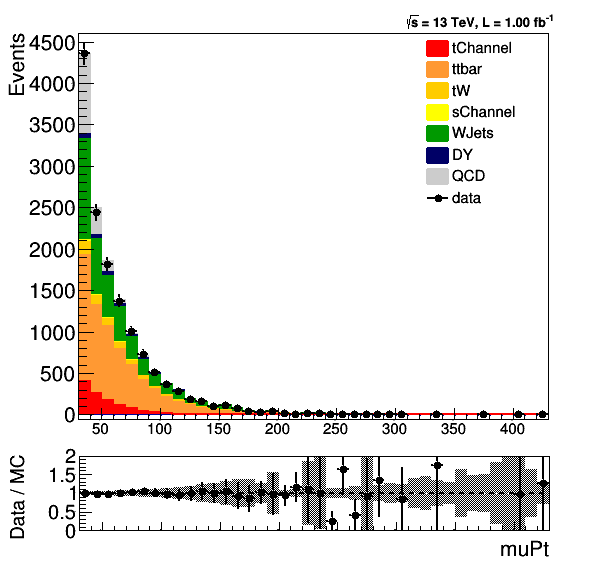
\includegraphics[width=0.48\textwidth]{figures/2J1T/muon_pt.png}
    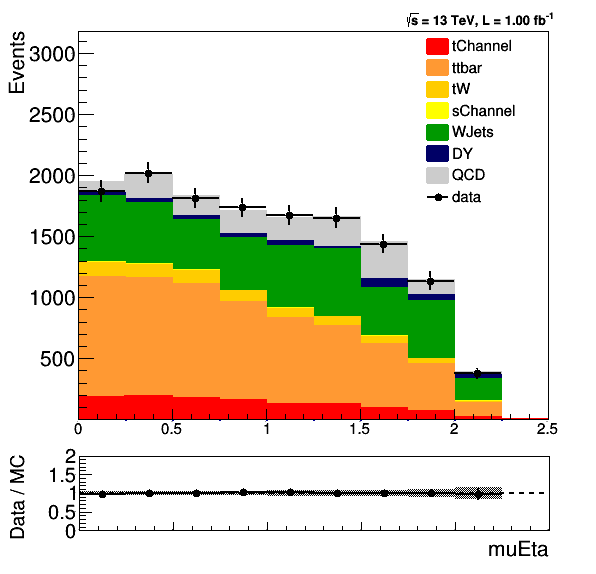
\includegraphics[width=0.48\textwidth]{figures/2J1T/muon_eta.png}
    \caption{\label{fig:2J1Tmu}{Left: $\mu$ \PT, Right: $\mu \eta$ in 2J1T category.}}
  \end{center}
\end{figure}


\begin{figure}[!Hhtb]
  \begin{center}
    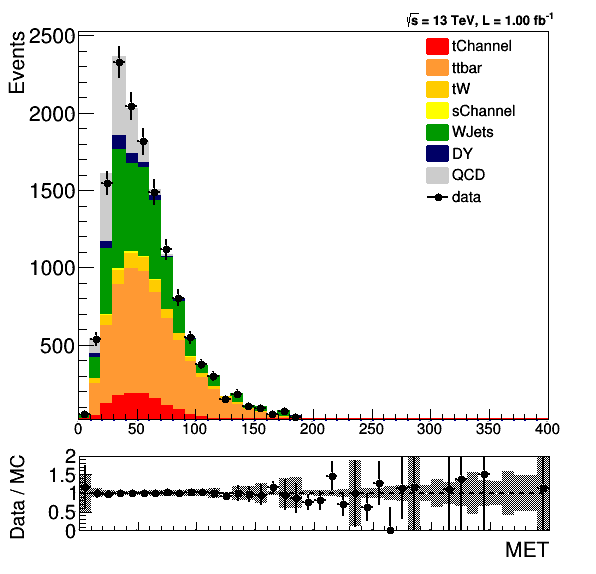
\includegraphics[width=0.48\textwidth]{figures/2J1T/MET.png}
    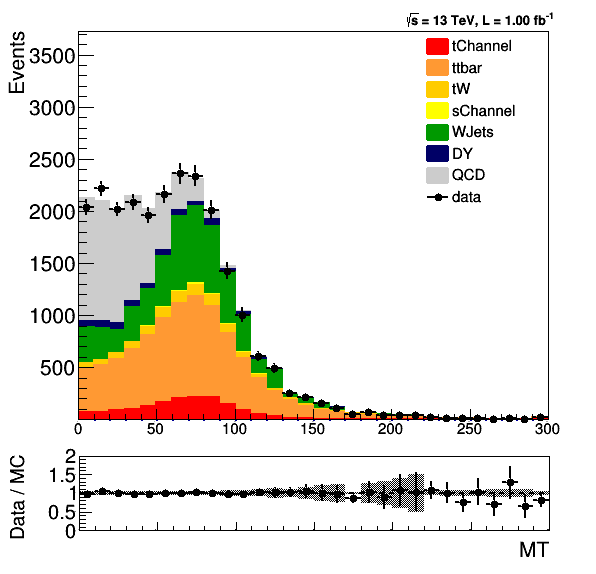
\includegraphics[width=0.48\textwidth]{figures/2J1T/MT.png}
    \caption{\label{fig:2J1TMETMT}{Left: \MET, Right: $M_T$ in 2J1T category.}}
  \end{center}
\end{figure}



\begin{figure}[!Hhtb]
  \begin{center}
    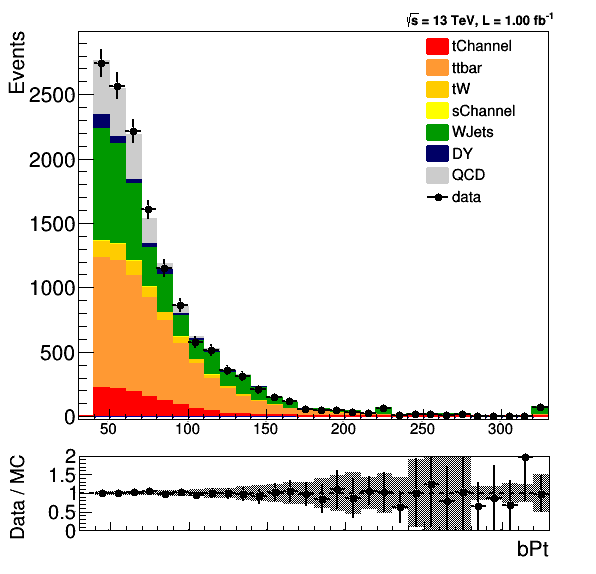
\includegraphics[width=0.48\textwidth]{figures/2J1T/bPt.png}
    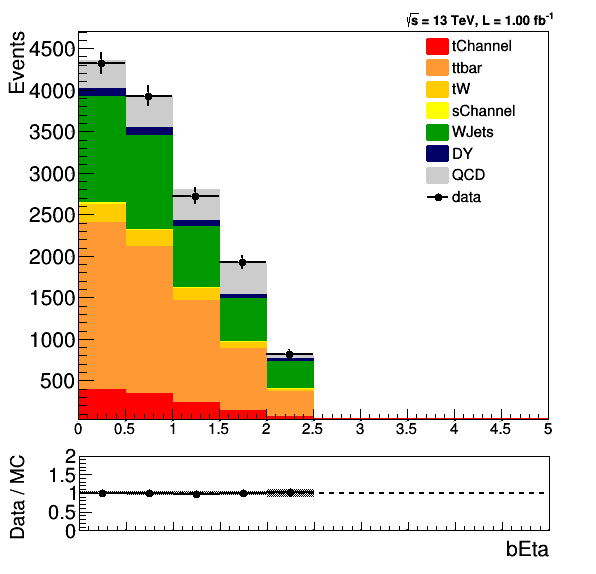
\includegraphics[width=0.48\textwidth]{figures/2J1T/b_eta.png}
    \caption{\label{fig:2J1TMETMT}{Left: \PT  Right: $\eta$ of the btagged jet in 2J1T category.}}
  \end{center}
\end{figure}

\begin{figure}[!Hhtb]
  \begin{center}
    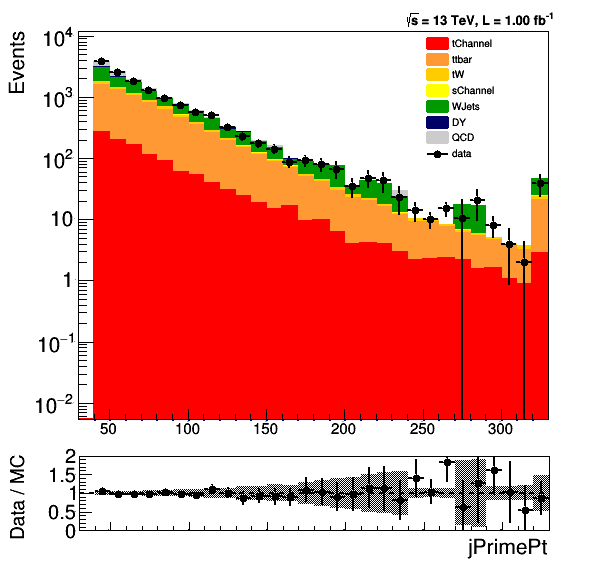
\includegraphics[width=0.48\textwidth]{figures/2J1T/jprime_pt.png}
    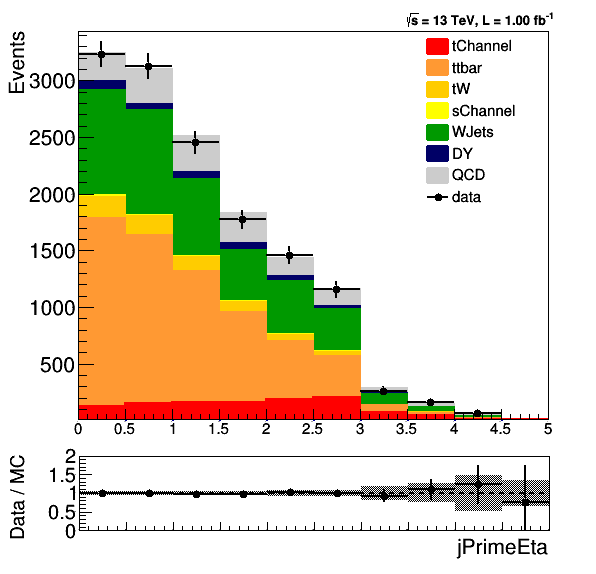
\includegraphics[width=0.48\textwidth]{figures/2J1T/jprime_eta.png}
    \caption{\label{fig:2J1TMETMT}{Left: \PT  Right: $\eta$ of the non-btagged jet in 2J1T category.}}
  \end{center}
\end{figure}




\begin{figure}[!Hhtb]
  \begin{center}
    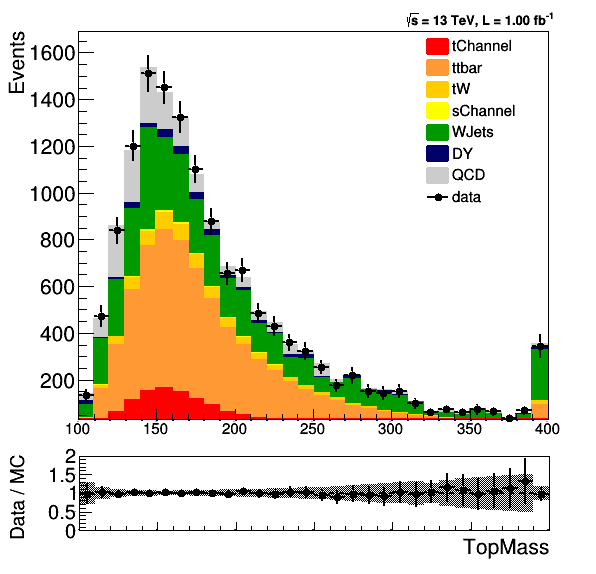
\includegraphics[width=0.48\textwidth]{figures/2J1T/TopMass.png}
    \caption{\label{fig:2J1TMETMT}{$m_{l\nu b}$ in 2J1T category.}}
  \end{center}
\end{figure}



%
%Amongst all the jet categories the 2Jets 1Tag sample has the best signal to background ratio for the t-channel. In this section we describe the additional cuts we perform in this sample and the sub-division of it in a Signal Region and Sideband Region.
%
%\subsection{Selection results}
%\label{sec:selresults}
%
%The number of selected events, step by step, leading to the 2J1T sample in data and simulation is shown in Tables ~\ref{tab:2J1T},~\ref{tab:2J1TEle}.
%The most dominating background is \tt, and the second is $\wjets$.
%One can clearly notice a discrepancy between data and simulation yields even after all cuts have been performed. 
%
%
%
%
%\clearpage
%\input{tab2J1T}
%\clearpage
%\input{tab2J1TEle}
%\clearpage
%
%
%%An interpretation to this result can be given considering the tagged jet multiplicity distributions in ~\ref{fig:nbjetPresel}:
%This is interpreted (see  also Refs.~\cite{AN-12-273,CMS-PAS-TOP-12-011}), as an excess of W+heavy flavours and the amonunt of this backround is estimated through data-driven techniques.
%
%In order to extract the inclusive cross section we perform an extra cut on the pt of the jets in the 2-jets 1-tag sample.
%This reduces the difference in shape of $\etalj$  due to the signal modeling, but reduces the available statistics by~half. 
%Studies have shown that this ends still up being convenient on the overall uncertainty. The last two columns of Tabb. ~\ref{tab:2J1T},
%~\ref{tab:2J1TEle} represent the number of events after this cut. The sample used for the charge ratio measurement is populated by the
%events in the second to last column of the same tables. 
%
%Figure~\ref{fig:2J1TtopMass}(a,b) show the reconstructed top mass $\topMass$ in the 2-jets 1-tag sample, variable used later on to define a $\wjets$ enriched region.
%
%	\begin{figure}[h]
%	  \begin{center}
%	    \subfigure[]{
%	    \includegraphics[width=0.48\textwidth]{figures/2J_1T_noSyst_topMass_MuStack.png}}
%	    \subfigure[]{
%	    \includegraphics[width=0.48\textwidth]{figures/2J_1T_noSyst_topMass_EleStack.png}}
%	    \caption{\label{fig:2J1TtopMass}{Distributions of $\mt$ in the 2Jets 1Tag sample (muons and electrons).}}
%	  \end{center}
%	\end{figure}
%
%
%
%
%\subsection{\wjets extraction}
%\label{sec:whfextraction}
%In order to keep the $\wjets$ contamination under control, an extra cut in $\topMass$ is performed in order to define a Signal Region(SR) for events which have
%$130 < \topMass < 220$. Events outside this region form the Sideband Region (SB). The discrepancy in the sideband region are attributed to $\wjets$. 
%One can extract a $\wjets$ distribution from the sideband subtracting the other background processes from the top mass sideband.
%A detailed description of the procedure can be found in Refs.~\cite{AN-12-273,CMS-PAS-TOP-12-011}.
%Figure ~\ref{fig:SRvsSBWJets} shows the agreement in the 2-jets 1-tag region between the $\wjets$ shape of the signal and sideband region 
%for muons and electrons with positive and negative charge. All the distributions yield a KS p-value of$ > 90\%$.
%We extract the $\wjets$ distribution from the sideband and we use simulation to get a bias and an uncertainty on this extratcion 
%using a procedure described in Sec.~\ref{sec:systematics}.
%Any $\ttbar$ mismodeling in the $|\eta| < 2.5$ region is kept into account with the reweighting procedure displayed in Sec.~\ref{sec:ttbar}.
%
%
%Tables ~\ref{tab:yield},~\ref{tab:yieldEle} show the nubmer of events in the signal and sideband regions for the muon and electron channel respectively. The 
%
%\begin{figure}[]
%\begin{center}
% \subfigure[]{
% \includegraphics[width=0.4\textwidth]{figures/MuSRSBPlus.png}}
% \subfigure[]{
% \includegraphics[width=0.4\textwidth]{figures/EleSRSBPlus.png}}\\
%%\caption{\label{fig:SRvsSBWJets}{Pseudorapidity distribution of light jets for the \wjets samples inside (red) and outside (blue) the $130<\topMass<220$ region, for muons (a), and electrons (b), positive charge.}}
%%\end{center}
%%\end{figure}
%%\begin{figure}[]
%%\begin{center}
% \subfigure[]{
% \includegraphics[width=0.4\textwidth]{figures/MuSRSBMinus.png}}
% \subfigure[]{
% \includegraphics[width=0.4\textwidth]{figures/EleSRSBMinus.png}}\\
%\caption{\label{fig:SRvsSBWJets}{Pseudorapidity distribution of light jets for the \wjets samples inside (red) and outside (blue) the $130<\topMass<220$ region, for muons (a,c), and electrons (b,d), positibe (a,b) and negative (c,d) charge.}}
%\end{center}
%\end{figure}
%
%
%\input{yieldTable}
%\input{yieldTableEle}
